In the MU-MIMO wireless context of interest, we have a MIMO transmitter with $N$ transmit antennas transmitting to $K$ single-antenna users. This topology means that the $i^{th}$ user has a  $N \times 1$ complex channel vector,$\underline{h}_i$, associated with it. That is, $\underline h_i\ \in \mathbb{C}^{1 \times N}$. A Rayleigh fading channel is assumed. Therefore each term in the channel vector $h_i$ follows a complex circularly symmetric iid normal distribution $\mathcal{N}_c(0,\frac{1}{N})$. It follows that the channel norm $\Vert \underline h_i \Vert^2$ follows a gamma distribution with the following parameters: $\Vert \underline h_i \Vert^2 \sim \mathcal{G}(2N,\frac{2}{N})$.

In order to formulate the problem as a sphere packing problem, channel vectors are assumed to be on the surface of a $N$-dimensional hyper-sphere in the complex domain, or a $2N$-dimensional hyper-sphere in the real domain. That is, the norms of each channel vector are assumed to be the same. This is evident from the definition of a hyper-sphere in $N$ dimensions:
\begin{equation}\label{eq:sphere_def}
    \begin{aligned}
        \mathcal{S}^{2N} = \lbrace \underline{h_i} \in \mathbb{R}^N \ : \ \Vert \underline{h_i} \Vert^2 = \rho \rbrace
    \end{aligned}
\end{equation}
where $\mathcal{S}^{2N}$ is the surface of a $2N$ hyper-sphere, $\underline{h}_i$ is a $N$-length complex vector that is being projected from the origin of the sphere, $\mathcal{O}$, to its surface, and $\sqrt{\rho}$ is the radius of the sphere. Without loss of generality, a sphere with radius of $\sqrt{\rho}$ can be mapped on a one-to-one basis to a sphere with radius $\rho$. Such a mapping is assumed for convenience.

In the case of a wireless channel experiencing deterministic path loss and Rayleigh fading, it is not practical to assume that all vectors have the same norm. If path loss is not exactly the same for each vector, the channel norms will differ between vectors (implying they would fall on the surface of spheres with different radii, or some other arbitrary shape). Similarly, the stochastic nature of the channel vectors, due to fading, will have the same effect.

However, if we assume channel state information at the transmitter (CSIT), the path loss can be estimated and accounted for (neglecting any estimation error in path loss, and assuming power control). Furthermore, the probability that $\Vert \underline{h_i} \Vert^2$ exists in the spherical shell defined by lower and upper radii, $\rho^-$ and $\rho^+$, respectively, is non-zero and can be easily calculated as a function of fading statistics and $\rho^-,\ \rho^+ $. An illustration of the members of this family of spheres is illustrated in Fig. $\ref{fig:concentric_sphere}$.

\begin{figure}
    \centering
    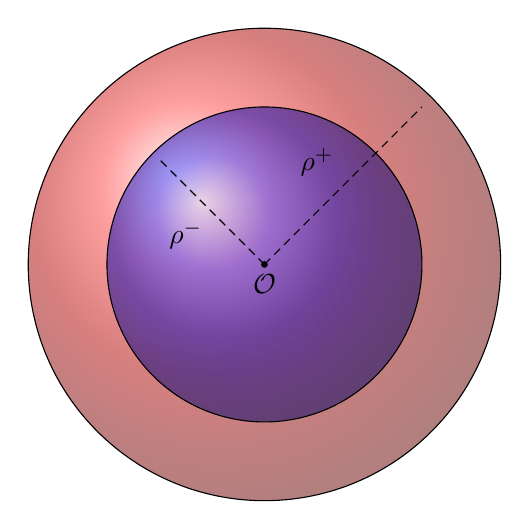
\begin{tikzpicture}
      \coordinate (O) at (0,0);
      
      % outer ball background color
      \shade[ball color = red, opacity = 0.5] (0,0) circle [radius = 3cm];
    
      %outer ball ball
      \draw (O) circle [radius=3cm];
    
      % inner ball background color
      \shade[ball color = blue, opacity = 0.5] (0,0) circle [radius = 2cm];
    
      % inner ball
      \draw (O) circle [radius=2cm];
      % label of ball center point
      \filldraw (O) circle (1pt) node[below] {$\mathcal{O}$};
    
      % radius for inner ball
      \draw[densely dashed] (O) to [edge label = $\rho^-$] (-1.33,1.33);
      % radius for outer ball
      \draw[densely dashed] (O) to [edge label = $\rho^+$] (2,2);
      
    
    \end{tikzpicture}
      \caption{Concentric hyper-spheres of radii $\rho^-,\rho^+$. Channel norms are restricted to this range in order to project vectors onto the surface of a hyper-sphere of constant radius. In order to pessimistically lower bound orthogonality probabilities, the larger radius of $\rho^+$ is chosen. The probability channel norms will fall into this range can be described in terms of channel fading statistics.}
    \label{fig:concentric_sphere}
\end{figure}
  
The CDF of the channel norm will be denoted by $F_{\Vert\underline{hi}\Vert^2}(m,\rho)$, where $\rho$ are realizations of the random variable formed by the channel norm. Each term in the $N$-length vector, $\underline{h}_i$ is represented by two iid normal random variables: one for the real part and one for the imaginary part. When forming the L2 norm of the $N$-length vector, each multiplication forms a sum of length four where each of the arguments of the sum are a product of two random variables. Namely, the sum takes the form real$\cdot$real + real$\cdot$imaginary + imaginary$\cdot$real + imaginary$\cdot$imaginary. Therefore we have a four-term sum of squared normal random variables. Therefore, this sum of squares results in a Gamma distribution with four degrees of freedom, the CDF of the resulting random variable becomes
\begin{equation}\label{eq:ch_sq_cdf_chan}
    \begin{aligned}
        F_{\Vert\underline{hi}\Vert^2}(\rho;m)& = \Gamma_n(2m,m\rho)\\
        &= Pr[\Vert\underline{h}_i\Vert^2 \leq \rho] \ \ ,
    \end{aligned}
\end{equation}
where $\Gamma_n(\cdot)$ is the incomplete normalized gamma function.

The probability that $\Vert\underline{h}_i\Vert^2$ lands in the shell between radii $\rho^+,\ \rho^-$,  is given by the subtraction of the respective CDF expressions:
\begin{equation}\label{eq:p_s}
    \begin{aligned}
        p_s = \Gamma_n(2N,N\rho^-) - \Gamma_n(2N,N\rho^+)
    \end{aligned}
\end{equation}

The issue of resolving the projection of channel vectors onto the surface of a sphere is still not entirely resolved: we have only described the probability the vectors will exist in a shell defined by upper and lower bounding radii. In order to pessimistically bound orthogonality analysis in the upcoming discussion, it is assumed that all the channel norms that exist in the shell are equal to $\rho^+$. This approach implies a trade-off between probability of channel norms existence and accuracy of orthogonality analysis: as ${(\rho^+-\rho^-)\rightarrow 0},\ p_s\rightarrow 0$; however, as  $(\rho^+-\rho^-)$ grows, so does the inaccuracy in orthogonality analysis.


